%%%%%%%%%%%%%%%%%%%%%%%%%%%%%%%%%%%%%%%%%
% Programming/Coding Assignment
% LaTeX Template
%
% This template has been downloaded from:
% http://www.latextemplates.com
%
% Original author:
% Ted Pavlic (http://www.tedpavlic.com)
%
% Note:
% The \lipsum[#] commands throughout this template generate dummy text
% to fill the template out. These commands should all be removed when 
% writing assignment content.
%
% This template uses a Perl script as an example snippet of code, most other
% languages are also usable. Configure them in the "CODE INCLUSION 
% CONFIGURATION" section.
%
%%%%%%%%%%%%%%%%%%%%%%%%%%%%%%%%%%%%%%%%%

%----------------------------------------------------------------------------------------
%	PACKAGES AND OTHER DOCUMENT CONFIGURATIONS
%----------------------------------------------------------------------------------------

\documentclass{article}

\usepackage{fancyhdr} % Required for custom headers
\usepackage{lastpage} % Required to determine the last page for the footer
\usepackage{extramarks} % Required for headers and footers
\usepackage[usenames,dvipsnames]{color} % Required for custom colors
\usepackage{graphicx} % Required to insert images
\usepackage{subcaption}
\usepackage{listings} % Required for insertion of code
\usepackage{courier} % Required for the courier font
\usepackage{lipsum} % Used for inserting dummy 'Lorem ipsum' text into the template
\usepackage{amsmath} % Use for multiple line equations
% Margins
\topmargin=-0.45in
\evensidemargin=0in
\oddsidemargin=0in
\textwidth=6.5in
\textheight=9.0in
\headsep=0.25in

\linespread{1.1} % Line spacing

% Set up the header and footer
\pagestyle{fancy}
\lhead{\hmwkAuthorName} % Top left header
\chead{\hmwkClass\ (\hmwkClassTime): \hmwkTitle} % Top center head
%\rhead{\firstxmark} % Top right header
\lfoot{\lastxmark} % Bottom left footer
\cfoot{} % Bottom center footer
\rfoot{Page\ \thepage\ of\ \protect\pageref{LastPage}} % Bottom right footer
\renewcommand\headrulewidth{0.4pt} % Size of the header rule
\renewcommand\footrulewidth{0.4pt} % Size of the footer rule

\setlength\parindent{0pt} % Removes all indentation from paragraphs

%----------------------------------------------------------------------------------------
%	CODE INCLUSION CONFIGURATION
%----------------------------------------------------------------------------------------

\definecolor{MyDarkGreen}{rgb}{0.0,0.4,0.0} % This is the color used for comments
\lstloadlanguages{Perl} % Load Perl syntax for listings, for a list of other languages supported see: ftp://ftp.tex.ac.uk/tex-archive/macros/latex/contrib/listings/listings.pdf
\lstset{language=Perl, % Use Perl in this example
        frame=single, % Single frame around code
        basicstyle=\small\ttfamily, % Use small true type font
        keywordstyle=[1]\color{Blue}\bf, % Perl functions bold and blue
        keywordstyle=[2]\color{Purple}, % Perl function arguments purple
        keywordstyle=[3]\color{Blue}\underbar, % Custom functions underlined and blue
        identifierstyle=, % Nothing special about identifiers                                         
        commentstyle=\usefont{T1}{pcr}{m}{sl}\color{MyDarkGreen}\small, % Comments small dark green courier font
        stringstyle=\color{Purple}, % Strings are purple
        showstringspaces=false, % Don't put marks in string spaces
        tabsize=5, % 5 spaces per tab
        %
        % Put standard Perl functions not included in the default language here
        morekeywords={rand},
        %
        % Put Perl function parameters here
        morekeywords=[2]{on, off, interp},
        %
        % Put user defined functions here
        morekeywords=[3]{test},
       	%
        morecomment=[l][\color{Blue}]{...}, % Line continuation (...) like blue comment
        numbers=left, % Line numbers on left
        firstnumber=1, % Line numbers start with line 1
        numberstyle=\tiny\color{Blue}, % Line numbers are blue and small
        stepnumber=5 % Line numbers go in steps of 5
}

% Creates a new command to include a perl script, the first parameter is the filename of the script (without .pl), the second parameter is the caption
\newcommand{\perlscript}[2]{
\begin{itemize}
\item[]\lstinputlisting[caption=#2,label=#1]{#1.pl}
\end{itemize}
}

%----------------------------------------------------------------------------------------
%	DOCUMENT STRUCTURE COMMANDS
%	Skip this unless you know what you're doing
%----------------------------------------------------------------------------------------

% Header and footer for when a page split occurs within a problem environment
\newcommand{\enterProblemHeader}[1]{
%\nobreak\extramarks{#1}{#1 continued on next page\ldots}\nobreak
%\nobreak\extramarks{#1 (continued)}{#1 continued on next page\ldots}\nobreak
}

% Header and footer for when a page split occurs between problem environments
\newcommand{\exitProblemHeader}[1]{
%\nobreak\extramarks{#1 (continued)}{#1 continued on next page\ldots}\nobreak
%\nobreak\extramarks{#1}{}\nobreak
}

\setcounter{secnumdepth}{0} % Removes default section numbers
\newcounter{homeworkProblemCounter} % Creates a counter to keep track of the number of problems
\setcounter{homeworkProblemCounter}{-1}

\newcommand{\homeworkProblemName}{}
\newenvironment{homeworkProblem}[1][Part \arabic{homeworkProblemCounter}]{ % Makes a new environment called homeworkProblem which takes 1 argument (custom name) but the default is "Problem #"
\stepcounter{homeworkProblemCounter} % Increase counter for number of problems
\renewcommand{\homeworkProblemName}{#1} % Assign \homeworkProblemName the name of the problem
\section{\homeworkProblemName} % Make a section in the document with the custom problem count
\enterProblemHeader{\homeworkProblemName} % Header and footer within the environment
}{
\exitProblemHeader{\homeworkProblemName} % Header and footer after the environment
}

\newcommand{\problemAnswer}[1]{ % Defines the problem answer command with the content as the only argument
\noindent\framebox[\columnwidth][c]{\begin{minipage}{0.98\columnwidth}#1\end{minipage}} % Makes the box around the problem answer and puts the content inside
}

\newcommand{\homeworkSectionName}{}
\newenvironment{homeworkSection}[1]{ % New environment for sections within homework problems, takes 1 argument - the name of the section
\renewcommand{\homeworkSectionName}{#1} % Assign \homeworkSectionName to the name of the section from the environment argument
\subsection{\homeworkSectionName} % Make a subsection with the custom name of the subsection
\enterProblemHeader{\homeworkProblemName\ [\homeworkSectionName]} % Header and footer within the environment
}{
\enterProblemHeader{\homeworkProblemName} % Header and footer after the environment
}

%----------------------------------------------------------------------------------------
%	NAME AND CLASS SECTION
%----------------------------------------------------------------------------------------

\newcommand{\hmwkTitle}{Assignment\ \#2} % Assignment title
\newcommand{\hmwkDueDate}{Friday,\ February\ 23,\ 2018} % Due date
\newcommand{\hmwkClass}{CSC411} % Course/class
\newcommand{\hmwkClassTime}{L2501} % Class/lecture time
\newcommand{\hmwkAuthorName}{Kaiyang Chen, Weixin Liu} % Your name

%----------------------------------------------------------------------------------------
%	TITLE PAGE
%----------------------------------------------------------------------------------------

\title{
\vspace{2in}
\textmd{\textbf{\hmwkClass:\ \hmwkTitle}}\\
\normalsize\vspace{0.1in}\small{Due\ on\ \hmwkDueDate}\\
\vspace{0.1in}
\vspace{3in}
}

\author{\textbf{\hmwkAuthorName}}
%\date{} % Insert date here if you want it to appear below your name

%----------------------------------------------------------------------------------------

\begin{document}

\maketitle
\clearpage

%----------------------------------------------------------------------------------------
%	PROBLEM 0
%----------------------------------------------------------------------------------------

\begin{homeworkProblem}
\noindent \textit{Download DataSet}
\\[5pt]
Two datasets are used in this project.
\\[5pt]
For \textit{Part 1} to \textit{Part 6}, this project works with MNIST dataset. It is a dataset of digits (0 to 9), which is avaiable at: http://yann.lecun.com/exdb/mnist/
\\[5pt]
For \textit{Part 8} to \textit{Part 10}, this project works with images of actors and actress. It is a subset from the FaceScrub website, which is available at: http://vintage.winklerbros.net/facescrub.html


\end{homeworkProblem}
\clearpage

%----------------------------------------------------------------------------------------
%	PROBLEM 1
%----------------------------------------------------------------------------------------

% To have just one problem per page, simply put a \clearpage after each problem

\begin{homeworkProblem}

\noindent \textit{Dataset description}
\\[10pt]
From Part 1 to 6, this project works with a dataset of digits (0 to 9). The total number of digits downloaded from the website is $70,000$. The dataset is pre-split into $60,000$ images in training set and $10,000$ images in the test set. Each image is $28 \times 28$-pixel. Those images may vary in boldness, font, and written style.
\\[5pt]
In Figure ~\ref{fig:part1}, 10 images of each of the digits is shown. It is evident that some of the digits may be hard to classify, even to humans. For example, the left-most $4$ can be interpreted as a $9$, the right-most $8$ can be read as a $1$. Moreover, the sixth $1$ from the left seems to be cut-off from the top. These particular examples may make the classification job harder and lower the accuracy, as we may see in later parts.
\\
\begin{figure*}[!ht]
\centering
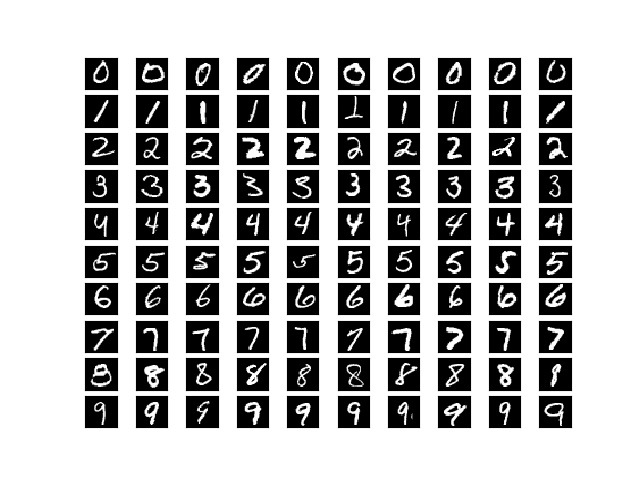
\includegraphics[width=1\linewidth, ]{Part1.jpg}
\caption{Visualizations of the digits dataset}
\label{fig:part1}
\end{figure*}
\\

\end{homeworkProblem}
\clearpage
%----------------------------------------------------------------------------------------
%	PROBLEM 2
%----------------------------------------------------------------------------------------

\begin{homeworkProblem}
\noindent \textit{Implement Forward Step}
\\[10pt]
The forward step of the neural network is implemented. The function \texttt{softmax(Y)} computes the softmax for the output neuron. The function \texttt{forward(X, W0b0)} computes the forward step of the neural network. In this implementation, the activation function is simply the linear combinations of the \textit{x}'s. The listing of the implementation is below:
\\[5pt]
\begin{lstlisting}
def softmax(Y):
	'''
	Return the output of the softmax function for the matrix of output Y. Y
	is an NxM matrix where N is the number of outputs for a single case, and M
	is the number of cases
	'''
	return exp(Y)/tile(sum(exp(Y),0), (len(Y),1))

def forward(X, W0b0):
	'''
	Function takes in X, the input, which is n*784 matrix, n being the 
	and W0b0, the weights matrix, which is a 785*10 matrix. The first 784 rows 
	corresponds to the neuron weights, the last row is the bias.
	Function returns the Output neurons O and the output after taking the 
	softmax function. 
	Both of the outputs have dimension 10*n.
	'''
	W0 = W0b0[:-1,:]
	b0 = W0b0[-1:,:].T
	O = dot(W0.T, X.T) + b0
	output = softmax(O)
	return O, output
\end{lstlisting}
\end{homeworkProblem}
\clearpage
%----------------------------------------------------------------------------------------
%	PROBLEM 3
%----------------------------------------------------------------------------------------

\begin{homeworkProblem}
\noindent \textit{Cost function of the neural network}
\\[10pt]
\noindent \textit{Part 3a)}
\\[10pt]
The gradient of the cost function with respect to the weight $w_{ij}$ is computed as follows. The final result is in Eq.~\ref{eq:3a_4}:
\\
The Cost function over all the training example is:
\begin{equation}
\label{eq:3a_1}
    Cost = -\sum_{k}\sum_{i}y_{i}^{(k)}logp_{i}^{(k)}
\end{equation} 
where Y is the label, P is the output prediction. k is the k-th data point (image), and i is the i-th pixel in one data point (image).
\\
The output prediction is computed using softmax function. 
\begin{equation}
\label{eq:3a_2}
    p_{i}^{(k)} = \frac{e^{o_{i}^{(k)}}}{\sum_{z}e^{o_{z}^{(k)}}}
\end{equation}

where i,k are defined same as above, O is the output neuron, and z is the z-th output neuron.
\\
The outout is computed using linear activation function.
\begin{equation}
\label{eq:3a_3}
    o_{i}^{(k)} = \sum_{j}w_{j,i}x_{j}^{(k)}+b_{i,k}
\end{equation}
where O is the output neuron, W is the weight, X is the input, b is bias. i, and k are defined same as above
\\
Now, the gradient of the cost function with respect to the weight is computed as follows.
\begin{equation}
\label{eq:3a_4}
\begin{split}
    \frac{\partial Cost}{\partial w_{i,j}} 
        & = \sum_{k} \frac{\partial Cost}{\partial O^{(k)}} \frac{\partial O^{(k)}}{\partial w_{i,j}} \\
        & = \sum_{k} (\sum_{i} \frac{\partial Cost}{\partial p_{i}^{(k)}} \frac{\partial p_{i}^{(k)}}{\partial o_{i}^{(k)}}) \frac{\partial o_{i}^{(k)}}{\partial w_{i,j}} \\
        & = \sum_{k} (p_{i}^{(k)} - y_{i}^{(k)}) x_{j}^{(k)}
\end{split}
\end{equation}
\\
Some of the steps above requires further justification by taking the partial derivatives of Eq.~\ref{eq:3a_1}, ~\ref{eq:3a_2}, and ~\ref{eq:3a_3}, see below:
$$\frac{\partial Cost}{\partial p_{i}^{(k)}} = -\frac{y_{i}^{(k)}}{p_{i}^{(k)}}$$
$$\frac{\partial p_{i}^{(k)}}{\partial o_{i}^{(k)}} = p_{i}^{(k)}(1-p_{i}^{(k)})$$
Thus we have:
$$(\sum_{i} \frac{\partial Cost}{\partial p_{i}^{(k)}} \frac{\partial p_{i}^{(k)}}{\partial o_{i}^{(k)}}) = (p_{i}^{(k)} - y_{i}^{(k)})$$ because only one of the $y_{i}$ is $1$ for each k, with all other $y_{i}$'s being zero. This equation is same as what we devired in class.
Finally,
$$\frac{\partial o_{i}^{(k)}}{\partial w_{i,j}} = x_{j}^{(k)}$$

\clearpage

\noindent \textit{Part 3b)}
\\[10pt]
The vectorized function to calculate the gradient of the cost function is implemented as follows. The function descriptions are written in the function comments. Function \texttt{CostFunction(X, Y, W0b0)}, \texttt{Gradient(X, Y, W0b0)} are used to compute the vectorized cost function gradient.
\\
\begin{lstlisting}
def CostFunction(X, Y, W0b0):
	'''
	Use Negative log-probabilities of all training cases as the cost function
	'''
	O, output = forward(X,W0b0)
	return -sum(Y*log(output))

def Gradient(X, Y, W0b0):
	'''
	Return Gradient of the cost function
	The first return matrix is the gradient w.r.t. the W0 matrix (weights), it has
	dimension 784 * 10
	The second return matrix is the gradient w.r.t. the b0 matrix (bias), it has
	dimension 10*1
	'''
	O, output = forward(X, W0b0)
	dy = output - Y
	return dot(dy, X).T, dot(dy, ones((X.shape[0],1)))

def finite_diff(CostFunction, X, Y, W0b0, row, col, h):
	'''
	Function for calculating one component of gradient using finite-difference 
	approximation. 
	h is the "small step" to take for the finite-difference
	row, col is the coordinate which that we wish to take the finite-differnce at
	'''
	W0b0_h = np.copy(W0b0)
	W0b0_h[row,col] = W0b0_h[row,col] + h
	return (CostFunction(X, Y, W0b0_h) - CostFunction(X, Y, W0b0))/h

def Check_diff(X, Y, W0b0, row, col ,h, gradW0, gradb0):
	'''
	This function prints the difference between gradient calculated using the
	finite difference method and vectorized gradient function
	'''
	finiteDiff = finite_diff(CostFunction, X, Y, W0b0, row, col ,h)
	if row == 784:
		print('The difference on Gradient_of_b0[%i, 0] is %010.10f' %(col, \
			abs(finiteDiff - gradb0[col,0])))
	else:
		print('The difference on Gradient_of_W0[%i,%i] is %010.10f' %(row, \
			col, abs(finiteDiff - gradW0[row,col])))

def part3b():
	'''
	Main function for part3b, in order to check the accuracy of the vectorized 
	gradient function by comparing to finite method
	7 Random points for each of the weights and the bias are selected from a 
	normal distribution of scale 0.0001.
	By setting row = 784, we are checking the gradients of the bias
	'''
	np.random.seed(1)
	W0 = np.random.normal(scale = 0.0001, size = (784,10))
	b0 = np.random.normal(scale = 0.0001, size = (10,1))
	W0b0 = np.vstack((W0, b0.T))
	row_ = np.random.randint(0,784,7) 
	#row = 784 # This indicates that we are checking for the gradient for b
	col_ = np.random.randint(0,10,7)
	h = 10**(-7)
	gradW0, gradb0 = Gradient(X_train, Y_train, W0b0)
	for i in range(7):
		Check_diff(X_train, Y_train, W0b0, row_[i], col_[i] ,h, \
			gradW0, gradb0)
		#Check_diff(X_train, Y_train, W0b0, row, col_[i] ,h, \
		#	gradW0, gradb0) #This indicates that we are checking for the gradint for b
\end{lstlisting}

The function \texttt{finite\_diff(CostFunction, X, Y, W0b0, row, col, h)}, \texttt{Check\_diff(X, Y, W0b0, row, col ,h, gradW0, gradb0)} and \texttt{part3b()} are then used to verify the accuracy by comparing the results from vectorized gradient and finite-method.\\
The Gradients of the Weights are checked:
\begin{lstlisting}
>>> part3b()
The difference on Gradient_of_W0[575,0] is 0.0001926810
The difference on Gradient_of_W0[165,3] is 0.0001806322
The difference on Gradient_of_W0[218,7] is 0.0000338211
The difference on Gradient_of_W0[627,2] is 0.0006195966
The difference on Gradient_of_W0[38,8] is 0.0005302735
The difference on Gradient_of_W0[378,3] is 0.0001368954
The difference on Gradient_of_W0[457,8] is 0.0002568140
\end{lstlisting}
The Gradients of the bias unit are checked:
\begin{lstlisting}
>>> part3b()
The difference on Gradient_of_b0[1, 0] is 0.0003257430
The difference on Gradient_of_b0[5, 0] is 0.0006381659
The difference on Gradient_of_b0[3, 0] is 0.0007544559
The difference on Gradient_of_b0[6, 0] is 0.0002933402
The difference on Gradient_of_b0[5, 0] is 0.0006381659
The difference on Gradient_of_b0[9, 0] is 0.0004366353
The difference on Gradient_of_b0[0, 0] is 0.0006255623
\end{lstlisting}

It is evident that these differences are smaller than $10^{-3}$. Therefore it is verified that the vectorized gradient function is accurate.

\end{homeworkProblem}
\clearpage


%----------------------------------------------------------------------------------------
%	PROBLEM 4
%----------------------------------------------------------------------------------------

\begin{homeworkProblem}
\noindent \textit{Training Neural Network without Momentum}
\\[10pt]
\noindent \textit{Choosing parameters}
\\[10pt]
The initial weights of the neural network is set to random variables in a scaled standard normal distribution with scale 0.0001. The initial weights cannot be all zeros, nor should it be too far away from zero. Therefore, a scaled standard normal distribution is chosen.
\\
The maximum iteration is set to be 1500. This is an arbitrary choice, but it is proven under 1500 iteration, the neural network has converged.(i.e. the performance has reached its plateau.)
\\
The learning rate $\alpha$ is chosen to be $1\times10^{-5}$. We chose this number because any alpha below or equal to $1\times10^{-4}$ makes the cost function diverge, i.e. the cost "blows up". Moreover, as in figure ~\ref{fig:part4_1}, the learning rate of $1\times10^{-5}$ is shown to be the one with lowest cost, i.e. it converges to minimum the fastest. Please note here is maximum number of iteration is $100$ which is different from the maximum iteration of the training, $1500$ because it is only use to justify the choice of $\alpha$. 
\\
\begin{figure*}[!ht]
\centering
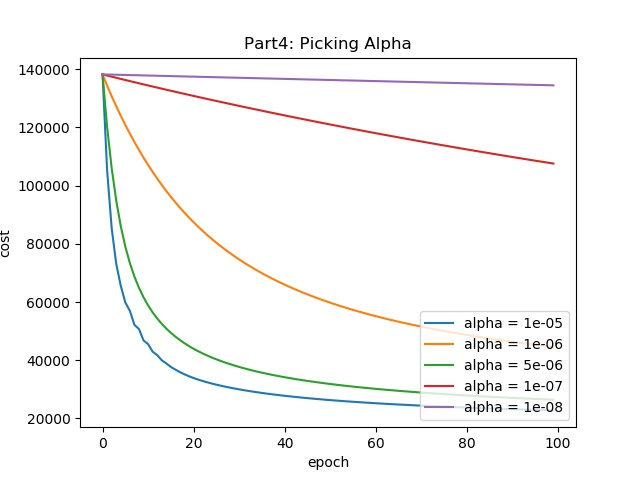
\includegraphics[width=1\linewidth, ]{part4_PickAlpha.jpg}
\caption{Cost function with different learning rate}
\label{fig:part4_1}
\end{figure*}
\\

\clearpage

\noindent \textit{Performance of neural network}
\\[5pt]
The learning curve of the training and testing set is shown in figure ~\ref{fig:part4_2}. The neural network "learns" in about 200 iterations And both of the training and testing set has a performance about $90\%$ 
\\
\begin{figure*}[!ht]
\centering
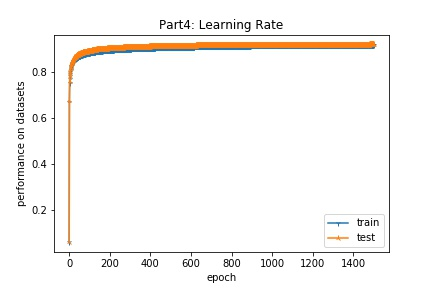
\includegraphics[width=1\linewidth, ]{part4_LearningRate.jpg}
\caption{Learning curve of the neural network}
\label{fig:part4_2}
\end{figure*}
\\

\clearpage

\noindent \textit{Visualize Weights}
\\[5pt]
The weights going into each of the output units (i.e. digits) are shown below in Figure ~\ref{fig:part4_3}.

\begin{figure*}[!ht]
\centering

\begin{subfigure}{.3\textwidth}
\centering
  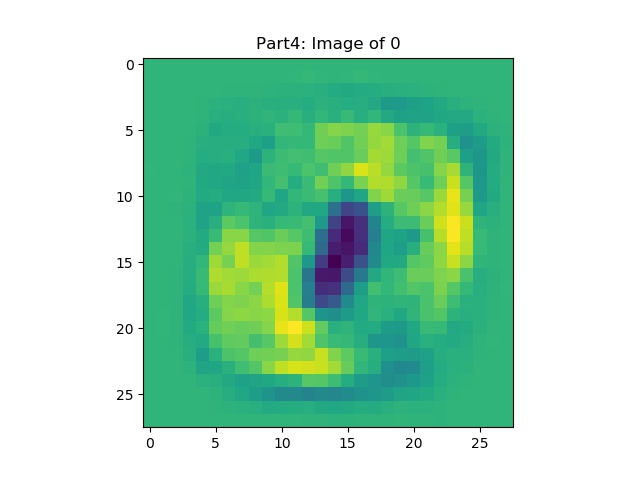
\includegraphics[width=1\linewidth]{part4_0.jpg}
  \caption{Weights of Output Neuron 0}
\end{subfigure}
\begin{subfigure}{.3\textwidth}
\centering
  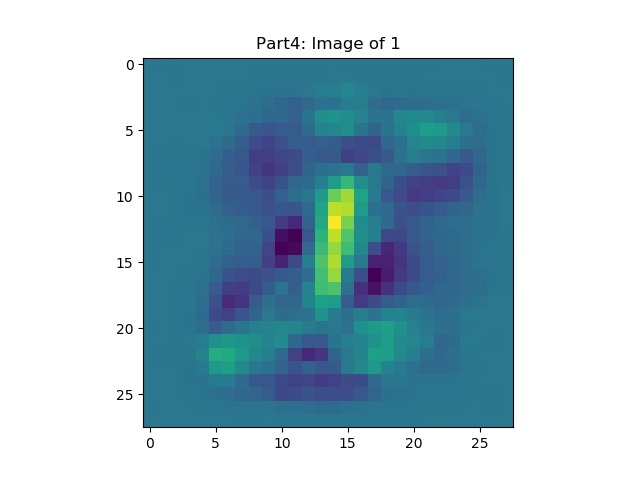
\includegraphics[width=1\linewidth]{part4_1.jpg}
  \caption{Weights of Output Neuron 1}
\end{subfigure}
\begin{subfigure}{.3\textwidth}
\centering
  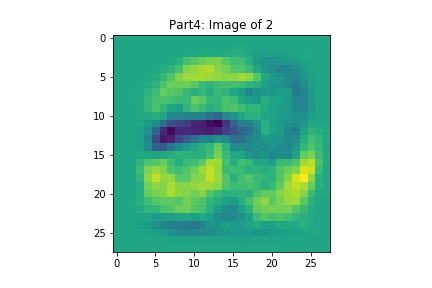
\includegraphics[width=1\linewidth]{part4_2.jpg}
  \caption{Weights of Output Neuron 2}
\end{subfigure}
\\
\begin{subfigure}{.3\textwidth}
\centering
  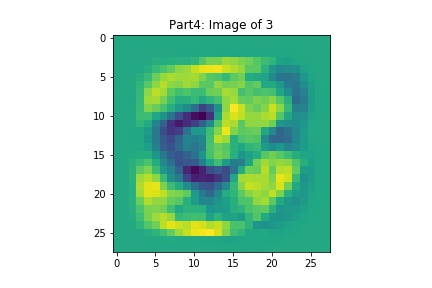
\includegraphics[width=1\linewidth]{part4_3.jpg}
  \caption{Weights of Output Neuron 3}
\end{subfigure}
\begin{subfigure}{.3\textwidth}
\centering
  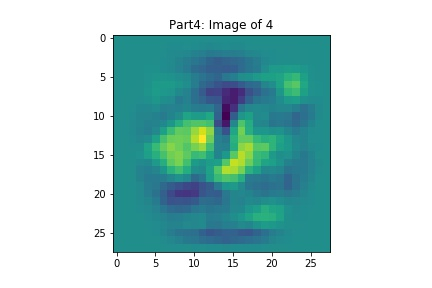
\includegraphics[width=1\linewidth]{part4_4.jpg}
  \caption{Weights of Output Neuron 4}
\end{subfigure}
\begin{subfigure}{.3\textwidth}
\centering
  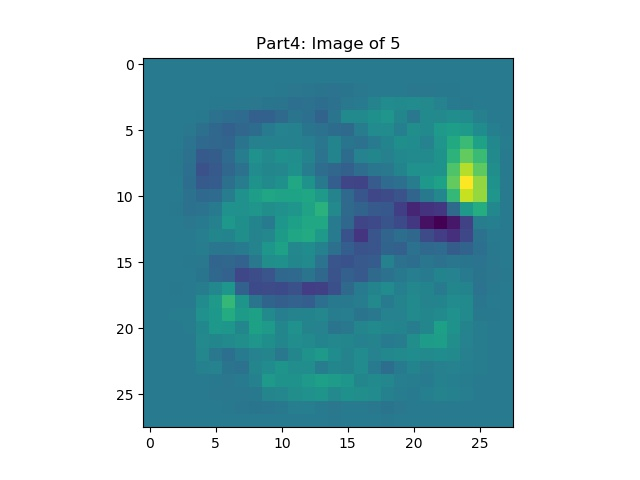
\includegraphics[width=1\linewidth]{part4_5.jpg}
  \caption{Weights of Output Neuron 5}
\end{subfigure}
\\
\begin{subfigure}{.3\textwidth}
\centering
  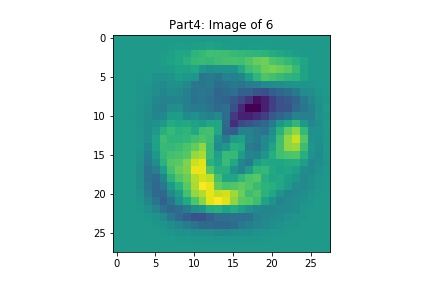
\includegraphics[width=1\linewidth]{part4_6.jpg}
  \caption{Weights of Output Neuron 6}
\end{subfigure}
\begin{subfigure}{.3\textwidth}
\centering
  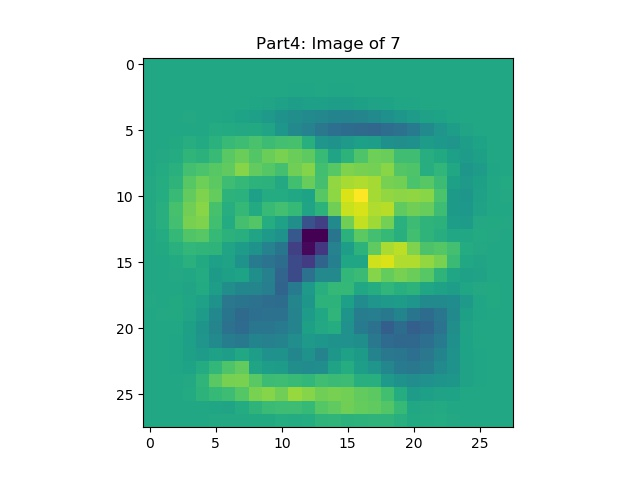
\includegraphics[width=1\linewidth]{part4_7.jpg}
  \caption{Weights of Output Neuron 7}
\end{subfigure}
\begin{subfigure}{.3\textwidth}
\centering
  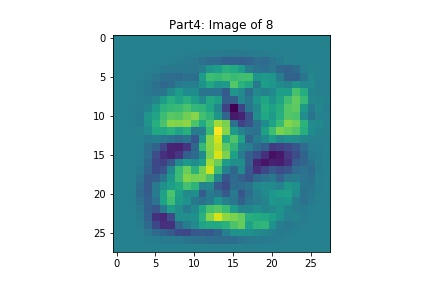
\includegraphics[width=1\linewidth]{part4_8.jpg}
  \caption{Weights of Output Neuron 8}
\end{subfigure}
\\
\begin{subfigure}{.3\textwidth}
\centering
  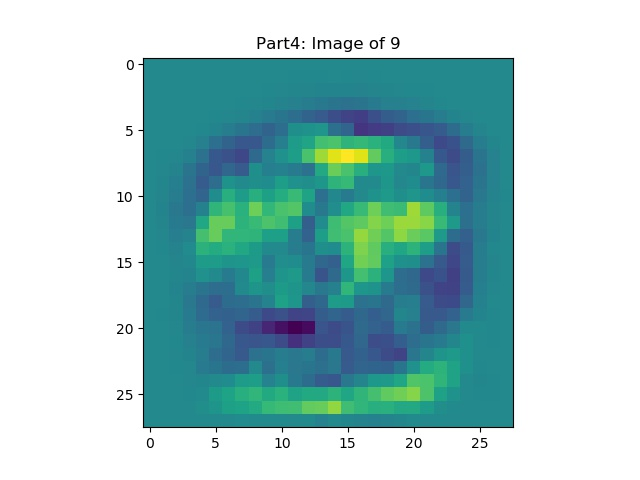
\includegraphics[width=1\linewidth]{part4_9.jpg}
  \caption{Weights of Output Neuron 9}
\end{subfigure}

\caption{Visualization of output units}
\label{fig:part4_3}
\end{figure*}

\end{homeworkProblem}
\clearpage




%----------------------------------------------------------------------------------------
%	PROBLEM 5
%----------------------------------------------------------------------------------------

\begin{homeworkProblem}
\noindent \textit{Training Neural Network with Momentum}
\\[5pt]
In this section, a momentum of $0.9$ is used. The parameter update rule for momentum is:
$$v \leftarrow \gamma v + \alpha \frac{\partial C}{\partial W}$$
$$W \leftarrow W - v$$
Where $\gamma$ is the momentum term, $\alpha$ is the learning rate and $W$ is the weights.
\\
The code implementation is below. Note that line 23 and 24 is the implementation of momentum. The function \texttt{CostFunction()} and \texttt{Gradient} are the same as the two functions in \textit{Part 3b)} of the same name.

\begin{lstlisting}
def grad_descent_part5(f, df, x, y, init_t, alpha, EPS=1e-5, max_iter=80000, \
 plotLR = False, gamma = 0.9):
	'''
	This function is same as the grad_descent function in part 4, except we update
	the weights with momentum term gamma.
	'''
	prev_t = init_t - 10 * EPS
	t = init_t.copy()
	iter = 0
	v = 0
	cost_func_ = []
	performanceTrain = []
	performanceTest = []
	while norm(t - prev_t) > EPS and iter < max_iter:
		costFunc = f(x, y, t)
		gradW0, gradb0 = df(x, y, t)
		grad = np.vstack((gradW0,gradb0.T))

		cost_func_.append(costFunc)
		performanceTrain.append(performance(x, y, t))
		performanceTest.append(performance(X_test,Y_test, t))
		prev_t = t.copy()
		v = gamma*v + alpha*grad
		t -= v
		if iter % 100 == 0:
			print "Iter", iter
			print "Cost", costFunc
			print "Gradient: ", grad, "\n"
		iter += 1
		
	if plotLR:
		fig = plt.figure(40)
		plt.title("Part5: Learning Rate")
		plt.xlabel('epoch')
		plt.ylabel('performance on datasets')
		plt.plot(range(iter),performanceTrain,'-1', label = 'train')
		plt.plot(range(iter),performanceTest,'-2', label = 'test')
		plt.legend(loc='lower right')
		fig.savefig(dirpath + '/part5_LearningRate.jpg')
		plt.show()

	return t, cost_func_, performanceTrain, performanceTest

def part5():
	'''
	Train the neural networking using gradient desecent.
	The initial weights is set to be a scaled standard normal with scale 0.0001
	The alpha is set to be 1e-5
	Maximum iteration is set to be 1500
	'''
	alpha = 1e-5
	np.random.seed(1)
	W0 = np.random.normal(scale = 0.0001, size = (784,10))
	b0 = np.random.normal(scale = 0.0001, size = (10,1))
	W0b0 = np.vstack((W0, b0.T))
	W0b0_part5, cost_func_part5, performanceTrain_part5, performanceTest_part5 = \
		grad_descent_part5(CostFunction, Gradient, X_train, Y_train, W0b0, alpha, \
		plotLR = True, max_iter = 1500)

	return W0b0_part5, cost_func_part5,	performanceTrain_part5, performanceTest_part5
\end{lstlisting}

\clearpage

The initialization of weights and setting of learning rate are the same as in part 4. The learning curve of training using momentum is shown below in Figure ~\ref{fig:part5_1}. To compare it with the previous training in \textit{Part 4} without momentum, a plot with smaller epoch is presented in Figure ~\ref{fig:part5_2}. From the plots, it is evident that training with momentum trains the neural network faster.

\begin{figure*}[!ht]
\centering
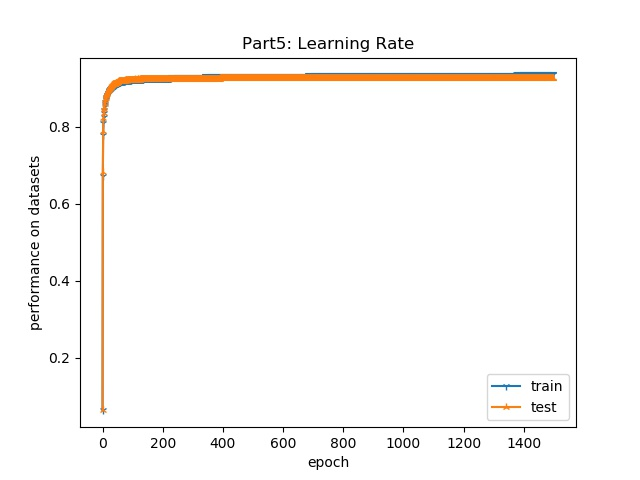
\includegraphics[width=0.7\linewidth, ]{part5_LearningRate.jpg}
\caption{Learning curve of the neural network, with momentum}
\label{fig:part5_1}
\end{figure*}

\begin{figure*}[!ht]
\centering
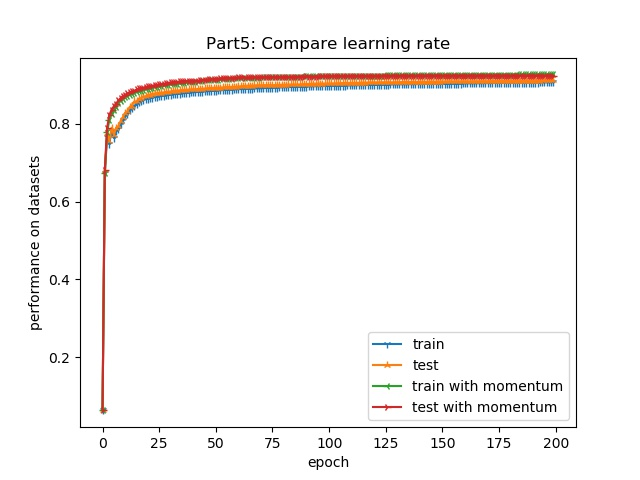
\includegraphics[width=0.7\linewidth, ]{part5_CompareLearn.jpg}
\caption{Comparison of learning curves between with and without momentum}
\label{fig:part5_2}
\end{figure*}

\end{homeworkProblem}
\clearpage


%----------------------------------------------------------------------------------------
%	PROBLEM 6
%----------------------------------------------------------------------------------------

\begin{homeworkProblem}
\noindent \textit{Part 6a) Contour Plot of the Cost Function}
\\[5pt]
To visualize cost function with different weights $w_1$ and $w_2$, a contour plot is produced in Figure ~\ref{fig:part6a_1}. The two weights chosen are the $249^{th}$ and $265^{th}$ pixel of the $9^{th}$ neuron, i.e. the digit $8$. A range from $-2$ to $2$ is chosen for both of the weights.

\begin{figure*}[!ht]
\centering
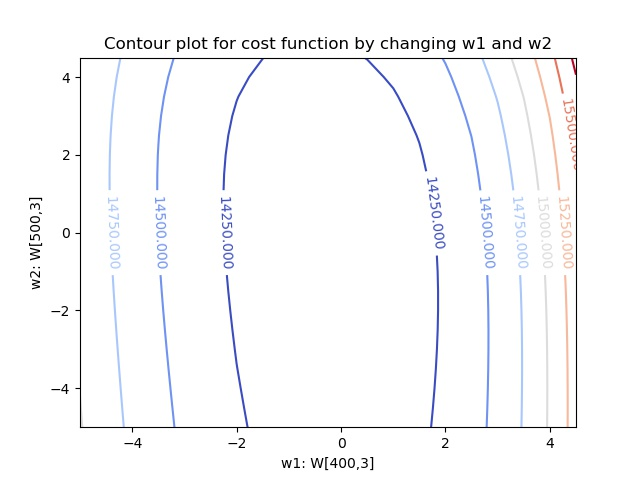
\includegraphics[width=0.55\linewidth, ]{part6_a.jpg}
\caption{Contour Plot of the Cost Function}
\label{fig:part6a_1}
\end{figure*}

\noindent \textit{Part 6b), c) Training using momentum}
\\[5pt]
To prove the use of momentum in some cases gives a better result. One specific example is given below in Figure ~\ref{fig:part6b_1}. We use the $300^{th}$ and $407^{th}$ pixel of the third neuron (i.e. digit $2$). The initialization of $w_1$ is $-2$ and $w_2$ is $0$. The learning rate for training without momentum is $3.8 \times 10^{-3}$ and the training with momentum is $4 \times 10^{-4}$. And the number of iteration is $10$.

\begin{figure*}[!ht]
\centering
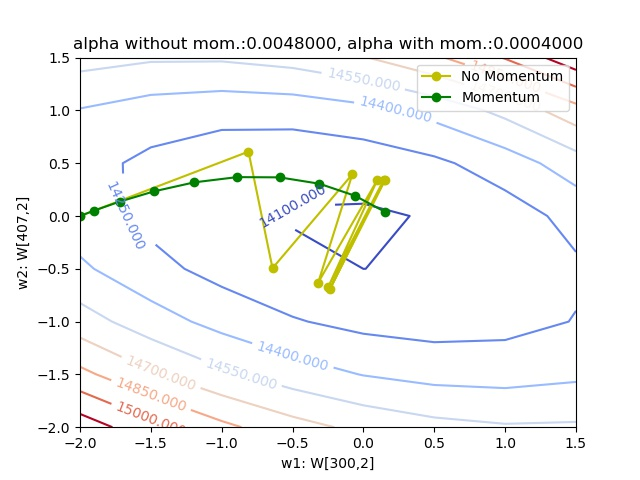
\includegraphics[width=0.55\linewidth, ]{part6_bc.jpg}
\caption{Comparing training with and without momentum}
\label{fig:part6b_1}
\end{figure*}

\clearpage
\noindent \textit{Part 6d) Difference between two trajectories}
\\[5pt]
The trajectory without momentum is very "bouncy", it has trouble going in the direction that can minimize the cost.
On the other hand, the trajectory with momentum is following the path that can minimize the cost better. The trajectory is smoother.
\\
This is because the cost function contour in this situation is a flat ellipse and the learning rate is big. It means when we start at a point closer to the major axis, in this case point (-2,0), the direction of no momentum training trajectory will keep changing because every movement changes it to a point with almost opposite gradient. On the other hand, the momentum training trajectory follows a smoother path because in each iteration, it moves further towards the minimum because of the "momentum".
\\[10pt]

\noindent \textit{Part 6e) When momentum fails to work}
\\[5pt]
Previously, in \textit{Part 6c)} and \textit{Part 6d)}, it is highlighted that a flat ellipse cost function contour with a initialization closer to the major axis which gives a big gradient change can demonstrate the effectiveness of momentum. 
\\
However, momentum can fail to work under certain situations such in Figure ~\ref{fig:part6e_1} below. In this case, the initialization of $w_1$ is $-0.5$ and $w_2$ is $-2$. The learning rate for training without momentum is $2 \times 10^{-3}$ and the training with momentum is $2 \times 10^{-4}$. And the number of iteration is $10$. We see that the no momentum trajectory goes into the minimum cost perfectly, whereas the momentum trajectory overshoots the minimum. This is because the initialization is along the minor access of the ellipse, thus the gradient is changes less, and points to the minimum more directly.

\begin{figure*}[!ht]
\centering
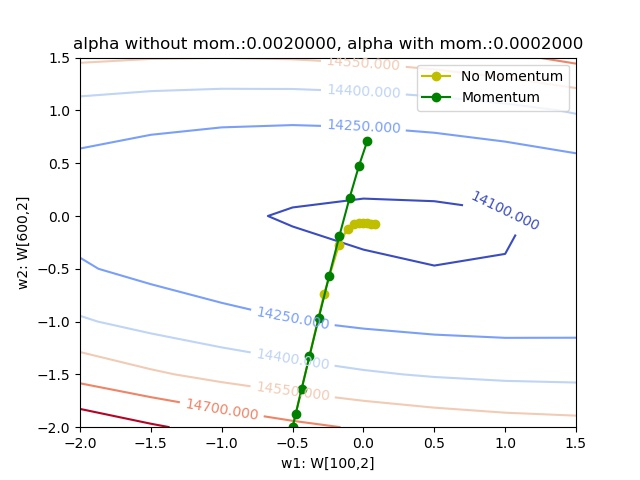
\includegraphics[width=0.55\linewidth, ]{part6_e.jpg}
\caption{Momentum Overshoot}
\label{fig:part6e_1}
\end{figure*}

Moreover, it is important to note that we deliberately avoid choosing pixels that are on the edges of the images because such pixels are usually dark and do not have any feature associated with them. As a result, the gradients on these pixels are small and there will not be any trajectories because the weights will not change at all.

\end{homeworkProblem}
\clearpage




%----------------------------------------------------------------------------------------
%	PROBLEM 7
%----------------------------------------------------------------------------------------

\begin{homeworkProblem}
\noindent \textit{}
Say we have a neural network with N layers each of which contains K neurons.\\
First, we define our symbols:
\begin{itemize}
    \item $\mathbf{W_{i}}$: K$\times$K matrix that represents the weights between the neurons on i-th layer and the neurons on (i+1)-th layer.
    \item $\mathbf{b_{i}}$: K $\times$ 1 vector that represents the bias of the i-th layer.
    \item $g_{i}$: the activation function used in neurons on i-th layer.
    \item $\mathbf{h_{i}}$: K $\times$ 1 vector that represents the neurons on i-th layer.
    \item $\mathbf{h_{i+1}} = g_{i+1}(\mathbf{W_{i}^{T}}\mathbf{h_{i}}+\mathbf{b_{i}})$
\end{itemize}
So we have:
\begin{itemize}
    \item the gradient between (i+1)-th layer and i-th layer: $\frac{\partial \mathbf{h_{i+1}}}{\partial\mathbf{h_{i}}} = \mathbf{W_{i}}g_{i+1}^{'}(\mathbf{W_{i}^{T}h_{i}+b_{i}})$
    \item the gradient between a layer and its weight matrix: $\frac{\partial \mathbf{h_{i}}}{\partial\mathbf{W_{i}}} = \mathbf{h_{i}}g_{i+1}^{'}(\mathbf{W_{i}^{T}h_{i}+b_{i}})$
    \item the gradient between a layer and its bias vector: $\frac{\partial \mathbf{h_{i}}}{\partial\mathbf{b_{i}}} = g_{i+1}^{'}(\mathbf{W_{i}^{T}h_{i}+b_{i}})$
\end{itemize}

Let's assume the complexity of element-wise operations(e.g. addition and multiplication) takes $O(1)$, so we have the complexity of matrix-wise operations:
\begin{itemize}
    \item matrix addition of two a$\times$b matrix is $O(ab)$
    \item matrix multiplication of a a$\times$b matrix and a b$\times$c matrix is $O(abc)$
    \item element-wise operations on a $a\times$b matrix is $O(ab)$
\end{itemize}

Start to evaluate the complexity of calculating gradients:
\begin{itemize}
    \item the gradient between a layer and its bias vector: $\frac{\partial \mathbf{h_{i}}}{\partial\mathbf{b_{i}}} = g_{i+1}^{'}(\mathbf{W_{i}^{T}h_{i}+b_{i}})$\\
    It requires a matrix multiplication of a K$\times$K matrix and a K$\times$1 matrix, a vector addition of two K$\times$1 matrices, and a element-wise operation with a K$\times$K matrix. Thus, the complexity is $ O(K^{2})+O(K)+O(K)= O(K^{2}) $.\\
    Note that this expression appears on other gradients, so we can store it and reuse.
    \item the gradient between (i+1)-th layer and i-th layer, $\frac{\partial \mathbf{h_{i+1}}}{\partial\mathbf{h_{i}}} = \mathbf{W_{i}}g_{i+1}^{'}(\mathbf{W_{i}^{T}h_{i}+b_{i}})$\\
    It requires a matrix multiplication of a K$\times$K matrix and a K$\times$1 matrix. Thus the complexity is $O(K^{2})$. (Note that $g_{i+1}^{'}(\mathbf{W_{i}^{T}h_{i}+b_{i}})$ is already calculated.)
    \item the gradient between a layer and its weight matrix: $\frac{\partial \mathbf{h_{i}}}{\partial\mathbf{W_{i}}} = \mathbf{h_{i}}g_{i+1}^{'}(\mathbf{W_{i}^{T}h_{i}+b_{i}})$\\
    It requires a matrix multiplication of a K$\times$1 matrix and a 1$\times$K matrix. Thus the complexity is $O(K^{2})$. (Note that $g_{i+1}^{'}(\mathbf{W_{i}^{T}h_{i}+b_{i}})$ is already calculated.)
\end{itemize}

In back propagation, assuming we stores all the intermediate values, we only need to compute: $\frac{\partial \mathbf{h_{i+1}}}{\partial\mathbf{b_{i}}}$ and $\frac{\partial \mathbf{h_{i}}}{\partial\mathbf{W_{i}}}$ N-1 times for N-1 connections between N layers, and $\frac{\partial \mathbf{h_{i+1}}}{\partial\mathbf{h_{i}}}$ N-2 times between N layers except for the input layer. Only consider one gradient calculation:
\begin{equation*}
    (N-1)(O(K^{2})+O(K^{2}))+(N-2)O(K^{2}) = O(NK^{2})
\end{equation*}

If compute each gradient individually without store intermediates steps, the cost of calculating gradients becomes:
\begin{equation*}
    \sum^{N}_{i=1}{\frac{\partial J}{\partial \mathbf{W_{i}}}}
\end{equation*}
For the sake of convenience, ignore the bias term and activation function:
\begin{align*}
    \frac{\partial J}{\partial{W_{i,j,k}}} &= \frac{\partial J}{\partial {h_{i+1,j}}}{h_{i,j}}^{'}\\
    &= \sum^{K}_{j_{i+2}}{\frac{\partial J}{\partial {h_{i+2,j_{i+2}}}}W_{i+1,j_{i+1},j_{i+2}}h_{i,j}^{'}}\\
    &= \sum^{K}_{j_{i+2}}\sum^{K}_{j_{i+3}}{\frac{\partial J}{\partial {h_{i+3,j_{i+3}}}}W_{i+2,j_{i+2},J_{i+3}}W_{i+1,j_{i+1},j_{2}}h_{i,j}^{'}}\\
    ... ...\\
    &= \sum^{K}_{j_{i+2}}\sum^{K}_{j_{i+3}} ... \sum^{K}_{j_{N}}{\frac{\partial J}{\partial {h_{N,j_{N}}}}W_{i+2,j_{i+2},j_{N-1}}... W_{i+1,j_{i+1},j_{i+2}}h_{i,j}^{'}}\\
\end{align*}

Assume all step takes $O(1)$, $\frac{\partial J}{\partial{W_{i,j,k}}}$ is $O(K^{N-i-1})$. Thus, the total complexity is:
\begin{align*}
KO(\frac{\partial J}{\partial {h_{N,j_{N}}}})+K^{2}O(\frac{\partial J}{\partial {W_{N-1,i,j}}})+K^{2}O(\frac{\partial J}{\partial {W_{N-2,i,j}}})+...+K^{2}O(\frac{\partial J}{\partial {W_{1,i,j}}})\\
=O(K)+O(K^{2})+O(K^{2})+O(K^{3})+...+O(K^{N}) = O(K^{N})
\end{align*}
So backpropagation has complexity of $O(NK^{2})$ while non-vectorized, non-storing calculation of gradient has complexity of O(K^{N})   
\end{homeworkProblem}
\clearpage



%----------------------------------------------------------------------------------------
%	PROBLEM 8
%----------------------------------------------------------------------------------------

\begin{homeworkProblem}
\noindent \textit{Training Faces Data using PyTorch}
\\[5pt]
For \textit{Part 8, Part 9} and \textit{Part 10}, the data set used is same as the ones used in \textit{Assignment 1}. The images used is a subset from the FaceScrub website, which is available at: 
\\
http://vintage.winklerbros.net/facescrub.html
\\[10pt]
\noindent \textit{Description of the System}
\\[5pt]
The architecture of the neural network is the following. There are $1024$ input neurons because we re-process the images to $32 \times 32$ pixel grey-scale. The first and only hidden layer has $12$ hidden units. The activation function on this hidden layer is \textit{tanh}. There are $6$ output neurons, because we have $6$ labels. There is no activation function on the output layer, only linear function is used. Finally, a softmax function is applied to the outputs. The optimizer function used is \texttt{torch.optim.Adam()}. The loss function used is cross-entropy.
\\
The input data is a randomly selected mini-batch of the whole training set after removing inappropriate images. The size of the batch is 10 images. Again, the inputs are $32 \times 32$ pixel grey-scaled images. Therefore the input is a $n\times1024$ matrix, with flattened images, not counting the bias unit.
\\
The initial weights of the neural network is random variables in a standard normal with a scale of $0.01$ (i.e. mean $0$, standard deviation $0.01$). The initial weights cannot be all zeros, nor should it be too far away from zero. Therefore, a scaled standard normal distribution is chosen.
\\
The learning rate $\alpha$ is $3\times10^{-4}$ and the maximum number of epoch is $1500$. 
\\
The learning curves is shown in ~\ref{fig:part8_1} below. Note that the training set performance is approaching to $100\%$ and the validation and testing set is about $85\%$. The final classfication performance on the test set is $86.67\%$

\begin{figure*}[!ht]
\centering
\includegraphics[width=0.9\linewidth, ]{{part8_32_10_1500_0.0003000}.jpg}
\caption{Learning curve of the neural network}
\label{fig:part8_1}
\end{figure*}

\clearpage

\noindent \textit{Choice of parameter}
\\[5pt]
Figures of learning rate using different parameter is shown in Figure \ref{fig:part8_tune} on the next page.
\\
The activation function used was \textit{tanh} because \textit{ReLU} gives a bad result as shown in Figure ~\ref{fig:part8_2} under all other parameters kept same.
\\
The learning rate $\alpha$ is choose to be $3\times10^{-4}$ because it gives the best result compared to $alpha = 1\times10^{-3}$ in Figure ~\ref{fig:part8_3} (this suggests that $\alpha$ could be larger) and $alpha = 5\times10^{-3}$ in Figure ~\ref{fig:part8_4} (this suggests that $\alpha$ might be too large because we see unstable behaviour).
\\
The size of mini-batch is 10 because with a mini-batch of 20 in Figure ~\ref{fig:part8_5}, the learning curve is the same. Also, we see that with a mini-batch of size 10, the training set performance is reaching $100\%$. But smaller mini-batch size is unreasonable because we have six distinct labels.
\\
The number of hidden neuron is chosen to be 12 because a 30 hidden neuron produces a similar performance, as shown in Figure ~\ref{fig:part8_6}. Increasing number of neuron increases the training time. Therefore we chose 12 hidden neurons to compromise between computation time and learning performance.
\\
The input photo is chosen to be $32\times32$ pixel because the input of $64\tiems64$ pixel gives slightly worse result, under all other parameter kept the same as the original setting, as shown in Figure ~\ref{fig:part8_7}.

\begin{figure*}[!ht]
\centering

\begin{subfigure}{.45\textwidth}
\centering
  \includegraphics[width=1\linewidth]{{part8_ReLU_32_10_1500_0.0003000}.jpg}
  \caption{Using ReLU as activation function}
  \label{fig:part8_2}
\end{subfigure}
\begin{subfigure}{.45\textwidth}
\centering
  \includegraphics[width=1\linewidth]{{part8_32_10_1500_0.0001000}.jpg}
  \caption{Learning rate = 0.0001}
  \label{fig:part8_3}
\end{subfigure}
\\
\begin{subfigure}{.45\textwidth}
\centering
  \includegraphics[width=1\linewidth]{{part8_32_10_1500_0.0005000}.jpg}
  \caption{Learning rate = 0.0005}
  \label{fig:part8_4}
\end{subfigure}
\begin{subfigure}{.45\textwidth}
\centering
  \includegraphics[width=1\linewidth]{{part8_32_20_1500_0.0003000}.jpg}
  \caption{Mini-batch size 20}
  \label{fig:part8_5}
\end{subfigure}
\\
\begin{subfigure}{.45\textwidth}
\centering
  \includegraphics[width=1\linewidth]{{part8_32_10_1500_0.0003000_30}.jpg}
  \caption{Hidden Neuron 30}
  \label{fig:part8_6}
\end{subfigure}
\begin{subfigure}{.45\textwidth}
\centering
  \includegraphics[width=1\linewidth]{{part8_64_10_1500_0.0003000_12}.jpg}
  \caption{Input photo $64\times64$ pixel}
  \label{fig:part8_7}
\end{subfigure}

\caption{Learning curves with different parameters}
\label{fig:part8_tune}
\end{figure*}

For the optimizer function, we have tried different optimizer functions, but they give similar performance.
\\
Finally, note that all other parameters, maximum epoch, the standard deviation of normal distribution initialization are educated choices. It is proven that these parameters gives a good performance, therefore no further tuning on these parameters.

\end{homeworkProblem}
\clearpage


%----------------------------------------------------------------------------------------
%	PROBLEM 9
%----------------------------------------------------------------------------------------

\begin{homeworkProblem}
\noindent \textit{Visualize Weights for useful hidden units}
\\[5pt]
For this part, we visualize the weights of hidden neurons that are useful for classifying Lorraine Bracco and Peri Gilpin. In order to accomplish this, we pick the four largest positive weights from hidden layer that is going into each of the two output neuron. After finding these positive weights and its associated neuron in the hidden layer, we then visualize them by plotting the weights of these hidden neurons.
\\
Figure ~\ref{fig:part9_1} shows the four most useful neurons for classifying Lorraine Bracco, which are: Neuron 3, 7, 10 and 11.
\\
Figure ~\ref{fig:part9_2} on next page shows the four most useful neurons for classifying Peri Gilpin, which are: Neuron 1, 2, 3 and 4.

\begin{figure*}[!ht]
\centering
\begin{subfigure}{.45\textwidth}
\centering
  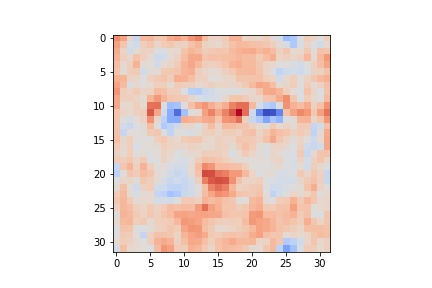
\includegraphics[width=1\linewidth]{part9_Bracco_3.jpg}
  \caption{Hidden Neuron 3}
\end{subfigure}
\begin{subfigure}{.45\textwidth}
\centering
  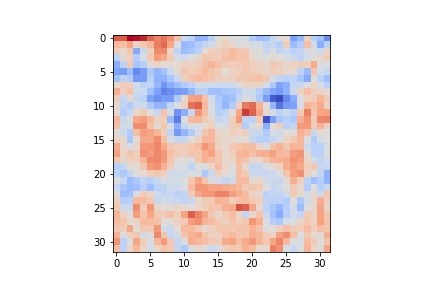
\includegraphics[width=1\linewidth]{part9_Bracco_7.jpg}
  \caption{Hidden neuron 7}
\end{subfigure}
\\
\begin{subfigure}{.45\textwidth}
\centering
  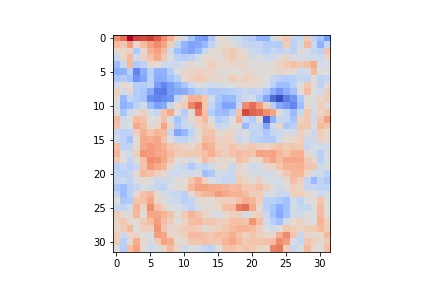
\includegraphics[width=1\linewidth]{part9_Bracco_10.jpg}
  \caption{Hidden neuron 10}
\end{subfigure}
\begin{subfigure}{.45\textwidth}
\centering
  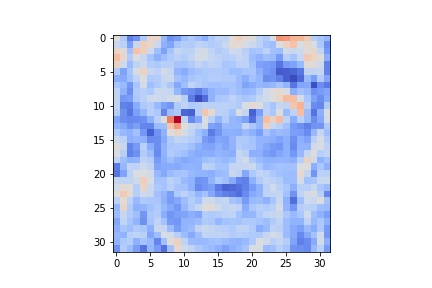
\includegraphics[width=1\linewidth]{part9_Bracco_11.jpg}
  \caption{Hidden neuron 11}
\end{subfigure}
\caption{Neurons useful for classifying Lorraine Bracco}
\label{fig:part9_1}
\end{figure*}


\begin{figure*}[!ht]
\centering
\begin{subfigure}{.45\textwidth}
\centering
  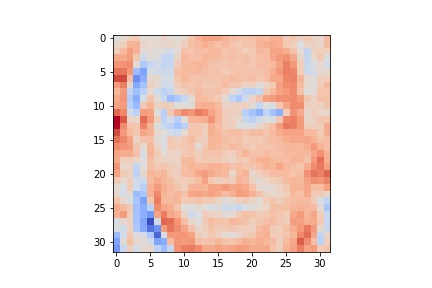
\includegraphics[width=1\linewidth]{part9_Gilpin_1.jpg}
  \caption{Hidden Neuron 1}
\end{subfigure}
\begin{subfigure}{.45\textwidth}
\centering
  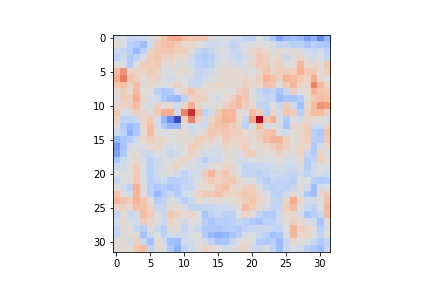
\includegraphics[width=1\linewidth]{part9_Gilpin_2.jpg}
  \caption{Hidden neuron 2}
\end{subfigure}
\\
\begin{subfigure}{.45\textwidth}
\centering
  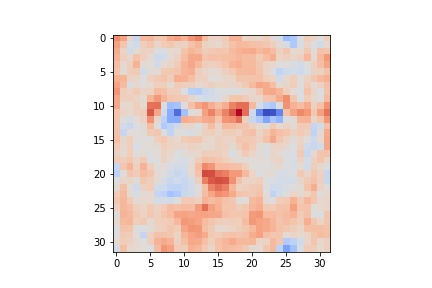
\includegraphics[width=1\linewidth]{part9_Gilpin_3.jpg}
  \caption{Hidden neuron 3}
\end{subfigure}
\begin{subfigure}{.45\textwidth}
\centering
  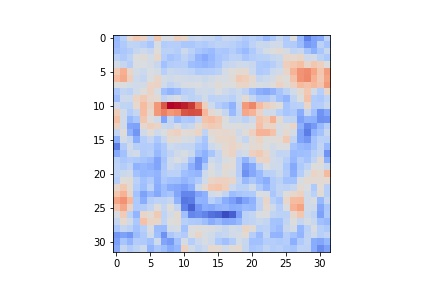
\includegraphics[width=1\linewidth]{part9_Gilpin_4.jpg}
  \caption{Hidden neuron 4}
\end{subfigure}
\caption{Neurons useful for classifying Peri Gilpin}
\label{fig:part9_2}
\end{figure*}

\end{homeworkProblem}
\clearpage


%----------------------------------------------------------------------------------------
%	PROBLEM 10
%----------------------------------------------------------------------------------------
\begin{homeworkProblem}
\noindent \textit{Training using AlexNet}
\\[5pt]
In this part, the value of activation at the last layer of the AlexNet is extracted and used as features to perform face classification. These modifications are performed inside the \texttt{class MyAlexNet(nn.Module)}, and it is included below.
\\
In particular, in line 10-14, we initialize the weights of the classifier to a random variables of a normal distribution with mean 0 and standard deviation 0.01. 
\\
In line 33-37, we add an additional fully-connected layer, which the activation function is just linear. This layer, which takes the activation values from the last layer of the AlexNet, is going to be our neural network that gets trained.
\\

\begin{lstlisting}
class MyAlexNet(nn.Module):
    def load_weights(self):
        an_builtin = torchvision.models.alexnet(pretrained=True)
        
        features_weight_i = [0, 3, 6, 8, 10]
        for i in features_weight_i:
            self.features[i].weight = an_builtin.features[i].weight
            self.features[i].bias = an_builtin.features[i].bias
        
        # Initilize weights
        classifier_weight_i = [0]
        for i in classifier_weight_i:
            self.classifier[i].weight.data.normal_(0.0,0.01)
            self.classifier[i].bias.data.normal_(0.0,0.01)

    def __init__(self, num_classes=1000):
        super(MyAlexNet, self).__init__()
        self.features = nn.Sequential(
            nn.Conv2d(3, 64, kernel_size=11, stride=4, padding=2),
            nn.ReLU(inplace=True),
            nn.MaxPool2d(kernel_size=3, stride=2),
            nn.Conv2d(64, 192, kernel_size=5, padding=2),
            nn.ReLU(inplace=True),
            nn.MaxPool2d(kernel_size=3, stride=2),
            nn.Conv2d(192, 384, kernel_size=3, padding=1),
            nn.ReLU(inplace=True),
            nn.Conv2d(384, 256, kernel_size=3, padding=1),
            nn.ReLU(inplace=True),
            nn.Conv2d(256, 256, kernel_size=3, padding=1),
            nn.ReLU(inplace=True),
            nn.MaxPool2d(kernel_size=3, stride=2),
        )
        # Addition of the extra layer, the linear function
        self.classifier = nn.Sequential(
            nn.Linear(256 * 6 * 6, 6),
            nn.Softmax()
        )
        
        self.load_weights()

    def forward(self, x):
        x = self.features(x)
        x = x.view(x.size(0), 256 * 6 * 6)
        x = self.classifier(x)
        return x

    # Exrtact the activation on the last layer
    def process_X(self, x):
        x = self.features(x)
        x = x.view(x.size(0), 256 * 6 * 6)
        return x.data.numpy()
\end{lstlisting}

The extraction of the activation value of the last layer of the AlexNet is done through the function \texttt{get\_data()}.\\
\begin{lstlisting}
def get_data(S, act, model, grayed = False, s = 0):
    act_rawdata = {}
    act_data = {}
    for i in act:
        act_rawdata[i] = np.empty((0,9216))
        act_data[i] = [0, 0, 0]

    for act_type in ['actors', 'actresses']:
        if grayed:
            dataset_path = dirpath + "/facescrub_%s_%i_grayed/" %(act_type, S[0])
        else:
            dataset_path = dirpath + "/facescrub_%s_%i/" %(act_type, S[0])
        for root, dirs, files in os.walk(dataset_path):
            dirs.sort()
            files.sort()
            for filename in files:
            
		        # extracting activation data of AlexNet
                im = imread(dataset_path + filename)[:,:,:3]
                im = im - np.mean(im.flatten())
                im = im/np.max(np.abs(im.flatten()))
                im = np.rollaxis(im, -1).astype(np.float32)
                im = Variable(torch.from_numpy(im).unsqueeze_(0), requires_grad=False)
                im = model.process_X(im)
                for i in act:
                    if i in filename:
                        act_rawdata[i] = np.vstack((act_rawdata[i], im))

    # randomly shuffle act_rawdata
    np.random.seed(s)
    for i in act:
        act_rawdata[i] = act_rawdata[i][np.random.permutation(act_rawdata[i].shape[0]),:]

    for i in act:
        act_data[i][0] = act_rawdata[i][:min(70, act_rawdata[i].shape[1] - 30),:]
        act_data[i][1] = act_rawdata[i][-30:-20,:]
        act_data[i][2] = act_rawdata[i][-20:,:]
    return act_data
\end{lstlisting}

It is important to note that we are only training the weights for output of AlexNet, i.e. the activation values. To make this point clear, we labeled these values as \texttt{self.classifier(x)}, as in line 44 of the first code snippet. And we train it using the code below by only calling \texttt{model.classifier(x)}:
\begin{lstlisting}
    for Epoch in range(nEpoch):
        for iMinibatch, Minibatch in enumerate(dataloader):
            x = Variable(Minibatch[:,:-1], requires_grad = False).type(dtype_float)
            y = Variable(Minibatch[:,-1], requires_grad = False).type(dtype_long)
            y_pred = model.classifier(x)
            loss = loss_fn(y_pred, y)
            model.classifier.zero_grad()  # Zero out the previous gradient computation
            loss.backward()    # Compute the gradient
            optimizer.step()   # Use the gradient information to make a step
\end{lstlisting}

\noindent \textit{Description of the system}
\\[5pt]
As previously mentioned, this neural network takes the activation values of AlexNet on the last layer. The inputs to the AlexNet is $227\times227\times3$ pixel RGB image. The activation values of AlexNet output has dimension $256\times6\times6 = 9126$. These values are used to train a fully connected neural network without hidden layers. A linear function is used to compute values for each of $6$ output neurons, because we have $6$ labels, each for one actor/actress. A softmax function is applied on top of the output neurons to reach the final values. (See line 34-37 of the first code snippet). 
\\
The optimizer used is \texttt{torch.optim.Adam}. The loss function used is cross-entropy.
\\
The learning rate used is $3\times10^{-4}$, and the batch-size is $10$, which are the same as those parameters in $Part 8$ because we wish to compare the performance. The maximum number of iteration is $600$, which is sufficient for this neural network to reach its best performance.
\\
The weights are initialized to a random variables of a normal distribution with mean 0 and standard deviation 0.01 because we try to avoid 0 weights but not having weights too far away from 0.

\clearpage

\noindent \textit{Performance of the System}
\\[5pt]
The performance is shown below in the learning curves in Figure ~\ref{fig:part10_1}. Compare to the performance of the previous neural network without using AlexNet in Figure ~\ref{fig:part8_1}, both the validation and test set performance has increased. The validation accuracy is high as $100\%$ and test accuracy is around $95\%$, compared to the around $85\%$ accuracy previously.

\begin{figure*}[!ht]
\centering
\includegraphics[width=0.9\linewidth, ]{{part10_227_10_600_0.0003000}.jpg}
\caption{Learning curve of the neural network with AlexNet}
\label{fig:part10_1}
\end{figure*}



\end{homeworkProblem}
\clearpage

%----------------------------------------------------------------------------------------

\end{document}